\usepackage{float}      % pentru [H]
\usepackage{subcaption}
\section{Experiment 2: 3D ResNet on Expanded Cohort (TTF1 \& CK7)}

\subsection{Rationale and Dataset Modification}
Following the initial proof-of-concept on 25 patients, the target biomarkers were adjusted due to data availability constraints. The scarcity of NAPSIN-positive samples necessitated a shift to predicting TTF1 and CK7 (Cytokeratin 7), markers crucial for distinguishing primary lung adenocarcinoma from metastatic carcinomas.

Consequently, the dataset was expanded to include a total of 87 patients.

\subsubsection{Data Distribution}
The dataset consists of 3D Computed Tomography (CT) scans and corresponding clinical labels. To ensure robust evaluation, a stratified split was performed based on the joint distribution of TTF1 and CK7 status (creating 4 distinct sub-groups).

\begin{itemize}
    \item \textbf{Total Patients:} 87
    \item \textbf{Stratification Key:} Combined TTF1/CK7 status (e.g., \texttt{TTF1\_1\_CK7\_0}).
    \item \textbf{Split Strategy:}
    \begin{itemize}
        \item \textbf{Train:} $\sim$62 patients
        \item \textbf{Validation:} $\sim$11 patients
        \item \textbf{Test:} $\sim$14 patients
    \end{itemize}
\end{itemize}

\subsection{Methodology: CT-Only 3D ResNet}

\subsubsection{Preprocessing Pipeline}
Unlike the initial experiment which relied heavily on external preprocessing scripts, this experiment integrated dynamic preprocessing using the \texttt{torchio} library directly within the training loop.
\begin{enumerate}
    \item \textbf{Volume Loading:} NIfTI files were loaded as \texttt{tio.ScalarImage} objects.
    \item \textbf{Spatial Normalization:} All volumes were resized or cropped/padded to a fixed target shape of \textbf{$(128, 128, 128)$}.
    \item \textbf{Intensity Normalization:} Voxel intensities were normalized based on the 1st and 99th percentiles to standardize Hounsfield Units (HU) across different scanners.
\end{enumerate}

\subsubsection{Model Architecture: 3D ResNet}
To capture spatial volumetric features without relying on engineered radiomics, a custom 3D ResNet architecture was designed using \texttt{TensorFlow/Keras}.

\begin{itemize}
    \item \textbf{Input:} $(128, 128, 128, 1)$ volumetric tensor.
    \item \textbf{Stem:} Initial Conv3D (16 filters, $7\times7\times7$ kernel) followed by BatchNormalization and MaxPooling3D.
    \item \textbf{Residual Body:}
    \begin{itemize}
        \item Three stages of residual blocks with increasing filter depth ($16 \rightarrow 32 \rightarrow 64$).
        \item Each block utilizes skip connections to mitigate the vanishing gradient problem and allow deeper feature extraction.
    \end{itemize}
    \item \textbf{Feature Aggregation:} GlobalAveragePooling3D converts the 3D feature maps into a dense vector.
    \item \textbf{Dual-Head Output:}
    \begin{itemize}
        \item The dense vector feeds into a shared dense layer (128 units) with Dropout (0.3).
        \item Two independent sigmoid output heads predict \textbf{TTF1} and \textbf{CK7} probabilities simultaneously.
    \end{itemize}
\end{itemize}

A lighter variant ("Light CT Model") using \texttt{SpatialDropout3D} and L2 regularization was also implemented to investigate overfitting tendencies observed in the deeper ResNet.

\subsection{Experimental Results}

\subsubsection{Training Configuration}
\begin{itemize}
    \item \textbf{Optimizer:} Adam ($LR=1e-4$).
    \item \textbf{Loss Function:} Binary Crossentropy (applied to both heads).
    \item \textbf{Batch Size:} 2 (due to memory constraints of 3D volumes).
    \item \textbf{Callbacks:} Early Stopping (patience=8) and ReduceLROnPlateau were used to monitor validation loss.
\end{itemize}

\subsubsection{Test Set Performance}
The model was evaluated on the held-out test set (n=14). The results indicate that the model struggles to generalize, likely due to the small sample size relative to the complexity of 3D volumetric data.

\textbf{Quantitative Metrics (Test Set):}
\begin{itemize}
    \item \textbf{CK7 AUC:} 0.53
    \item \textbf{TTF1 AUC:} 0.45
    \item \textbf{TTF1 Accuracy:} 0.71 (Driven by majority class prediction)
    \item \textbf{CK7 Accuracy:} 0.54
\end{itemize}

\begin{figure}[H]
    \centering
    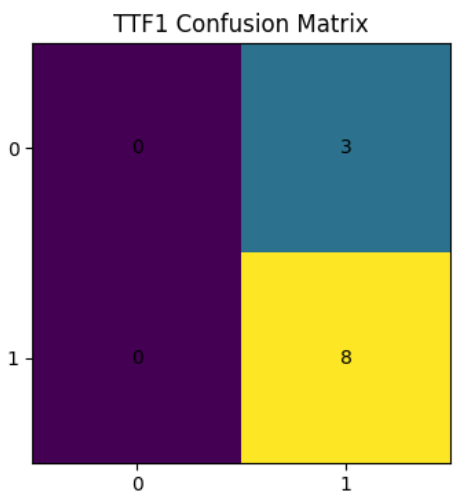
\includegraphics[width=0.5\textwidth]{image_2025-11-19_173106760.png}
    \caption{Confusion Matrix for TTF1.}
    \centering
    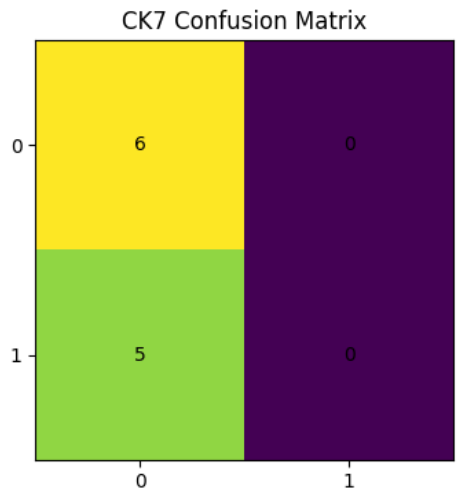
\includegraphics[width=0.5\textwidth]{image_2025-11-19_173213575.png}
    \caption{onfusion Matrix for CK7.}
\end{figure}



\subsubsection{Conclusion of Experiment 2}
While the dataset size was increased to 87 patients, training a 3D ResNet solely on raw pixel data proved difficult. The model converged to predicting the majority class distribution, resulting in AUC scores near 0.5 (random guessing). 

The lack of explicit feature engineering (Radiomics) in this specific run suggests that for datasets of this magnitude ($N < 100$), deep learning models struggle to extract meaningful biological signals from raw 3D volumes alone without the guidance of radiomics features or significantly stronger regularization/pre-training.